%%%%%%%%%%%%%%%%%%%%%%%%%%%%%%%%%%%%%%%%%%%%%%%%%%%%%%%%%%%%%%%%%%%%%%
%     File: ExtendedAbstract_resul.tex                               %
%     Tex Master: ExtendedAbstract.tex                               %
%                                                                    %
%     Author: Andre Calado Marta                                     %
%     Last modified : 27 Dez 2011                                    %
%%%%%%%%%%%%%%%%%%%%%%%%%%%%%%%%%%%%%%%%%%%%%%%%%%%%%%%%%%%%%%%%%%%%%%
% Results
% Results should be clear and concise.
% Discussion
% This should explore the significance of the results of the work, not
% repeat them. A combined Results and Discussion section is often
% appropriate. Avoid extensive citations and discussion of published
% literature.
%%%%%%%%%%%%%%%%%%%%%%%%%%%%%%%%%%%%%%%%%%%%%%%%%%%%%%%%%%%%%%%%%%%%%%
\subsection{Mean field}
\label{sec:resul}
In Fig.(\ref{fig:nanoGraphVsTMD}), we compare the magnetization profile along the rows of the ribbon (the transverse direction) for graphene nanoribbon with the same profile obtained for a TMD nanoribbon.

In Fig.(\ref{fig:bandsU20}), we present the spin-resolved band structure within the ordered phase of a TMD nanoribbon of width $N_y = 16$.
The first two aspects to notice are that spin degeneracy has been lifted, and that the shape of the bands has been distorted.
The part of the bands near the Fermi energy $\varepsilon_F$ determines the physics of the phase.
The interplay between the geometry of the tight-binding model, its parameters, the on-site interaction and temperature gives rise to different phases since it determines the shape of the bands and the location of the Fermi energy corresponding to charge neutrality.
Two changes with respect to the free bands are crucial:
the K-point splitting (circled in yellow), corresponding to a region where one of the bands stays below the Fermi energy, while the other stays above - this leads to spin polarization of the eigenstates associated with these energies; the band crossing (circled in green) - as $U$ varies, and the bands move upward or downward, and eventually distort, the states around this band crossing become either occupied or unoccupied, and since two opposite spin bands meet (\emph{at right angles}) at this point, this will lead to the appearance of a magnetization with with a magnitude that depends on the point in $k$ where the two bands meet.
\begin{figure}[H]
\centering
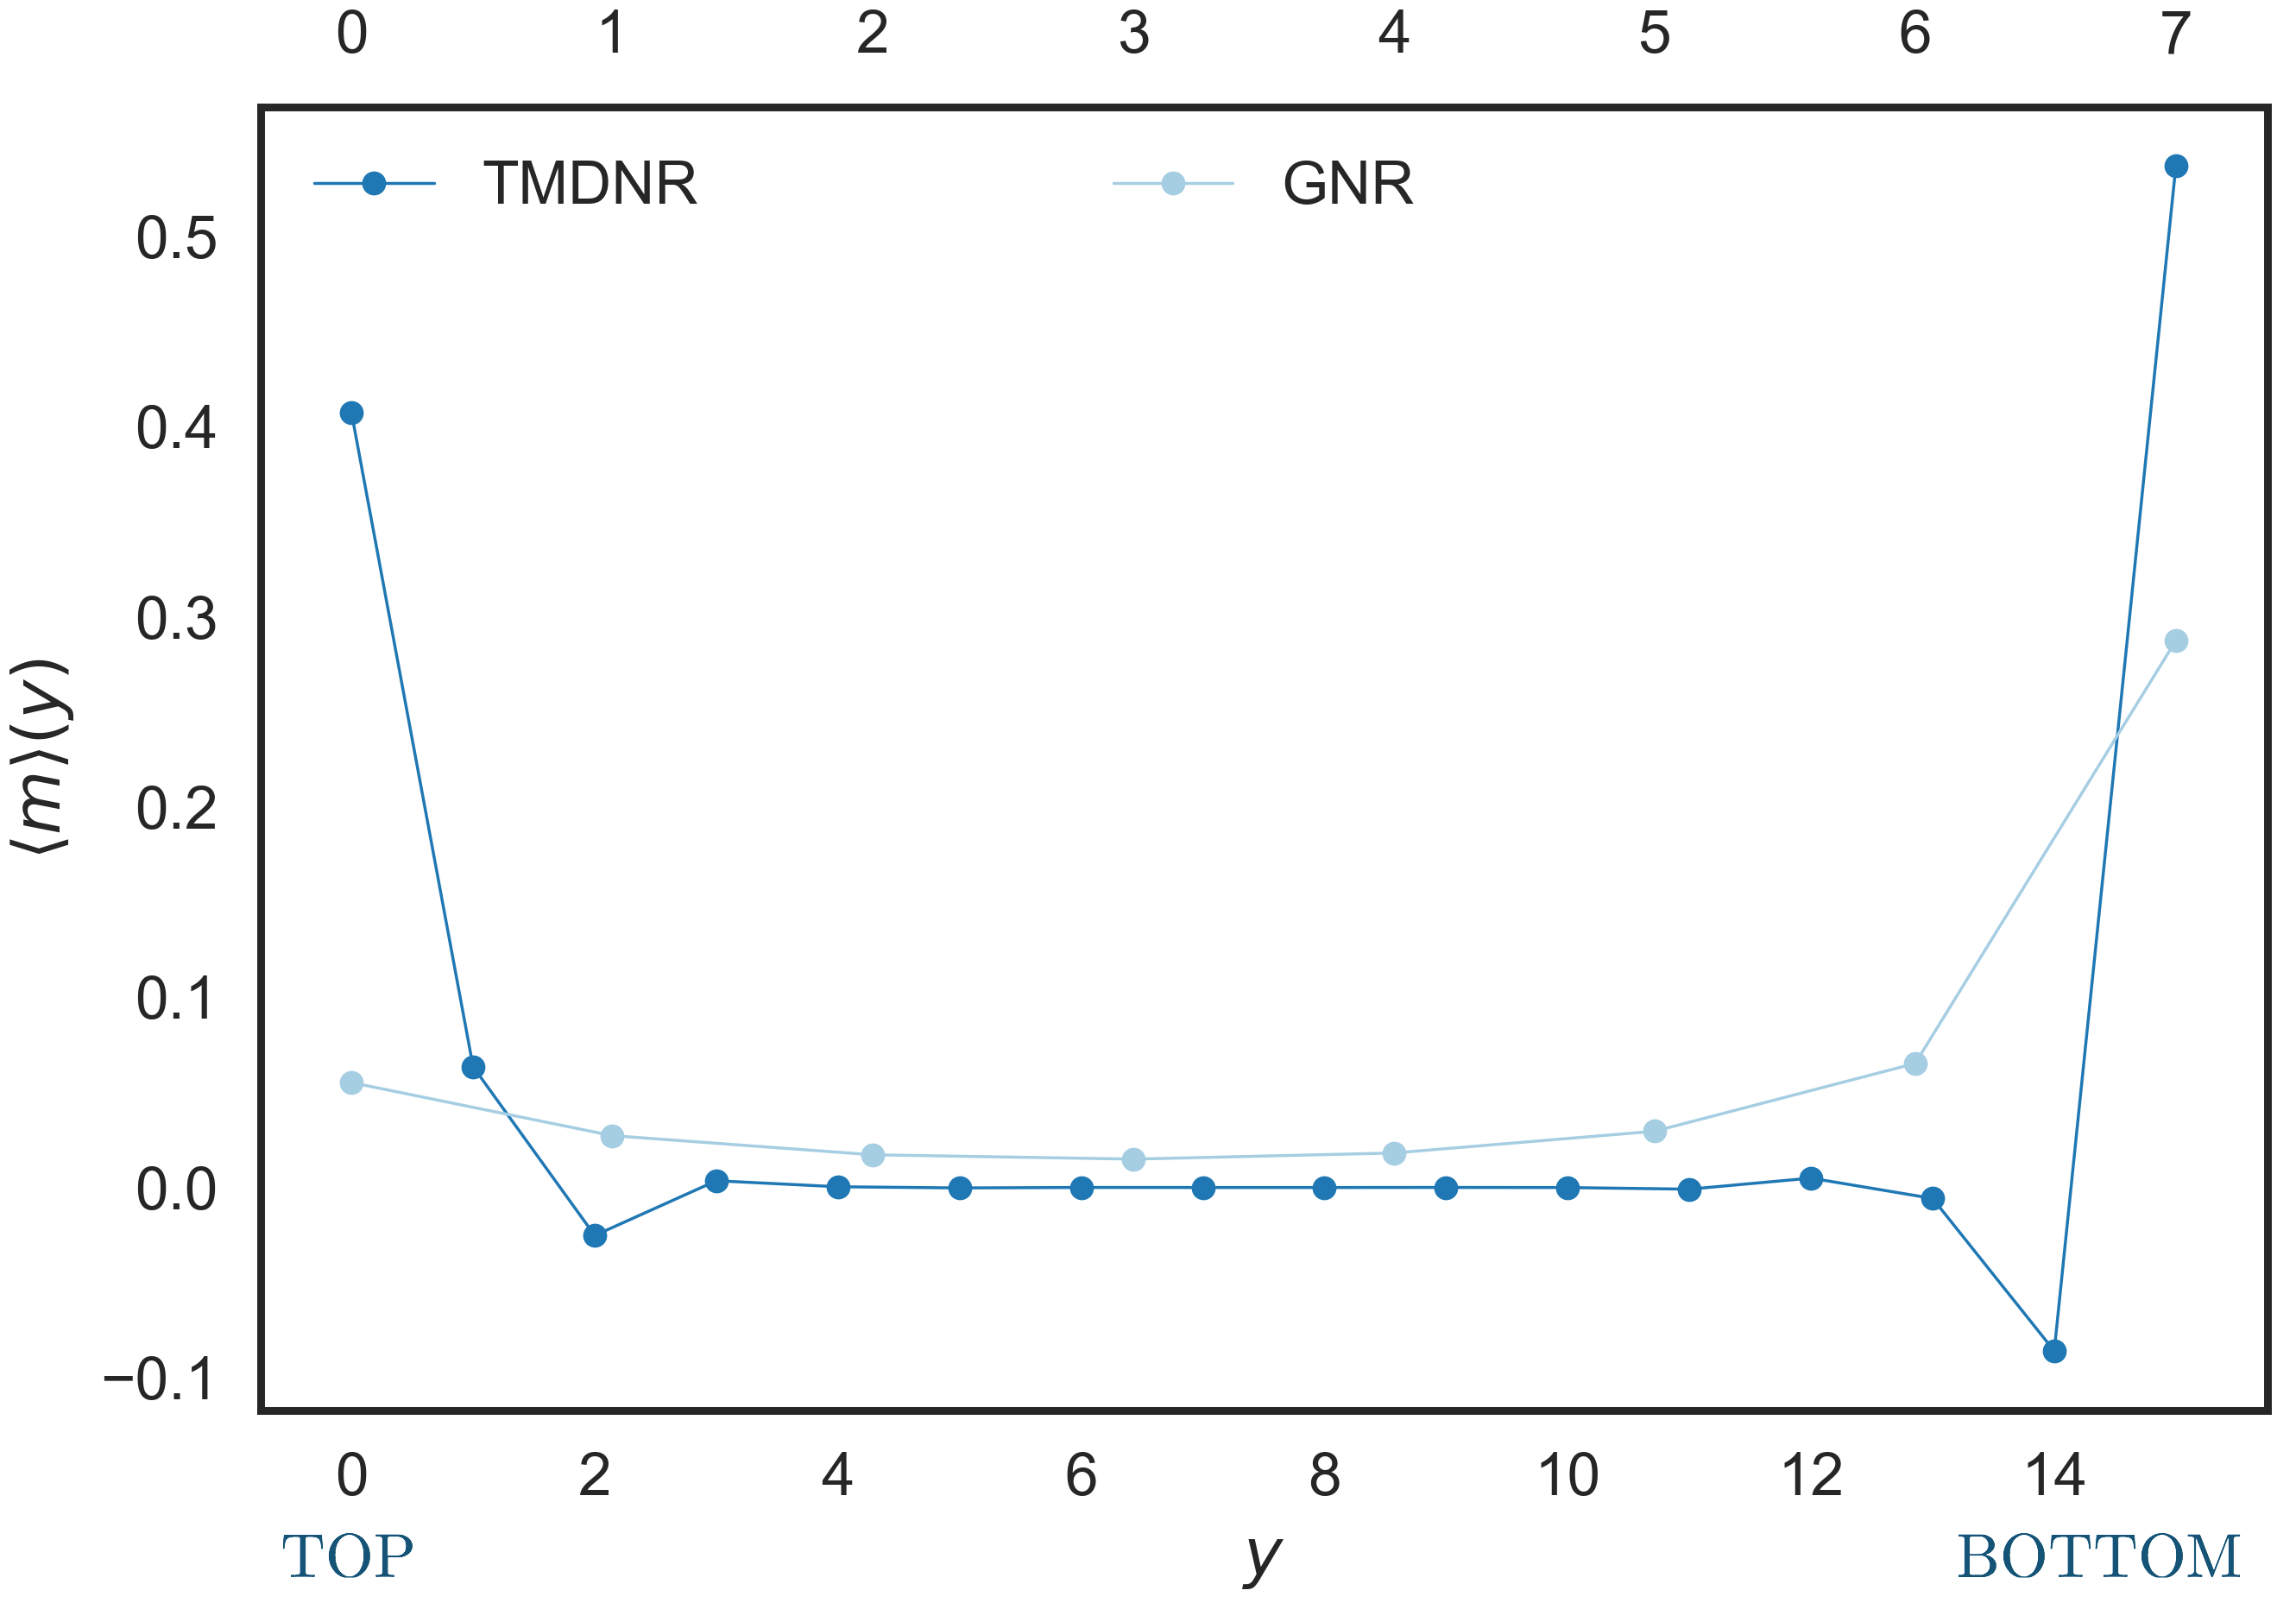
\includegraphics[scale=0.55]{images/magProf.png}
	\caption{Ordered phases.
	Spin density profile along the ribbon's transverse direction $\left\langle m \right\rangle (y)$ for the Hubbard model at half filling ($\left\langle n \right\rangle = 1$) for a $16 \times 8$ graphene nanoribbon (GNR) at $U=1.2t$ (left) and a TMDNR with $N_y = 16$ at $U = 20| t_0 |$, and electron density $\left\langle n \right\rangle = 0.66$, the filling that corresponds to charge neutrality.}
	\label{fig:nanoGraphVsTMD}
\end{figure}
\begin{figure}[H]
\centering
    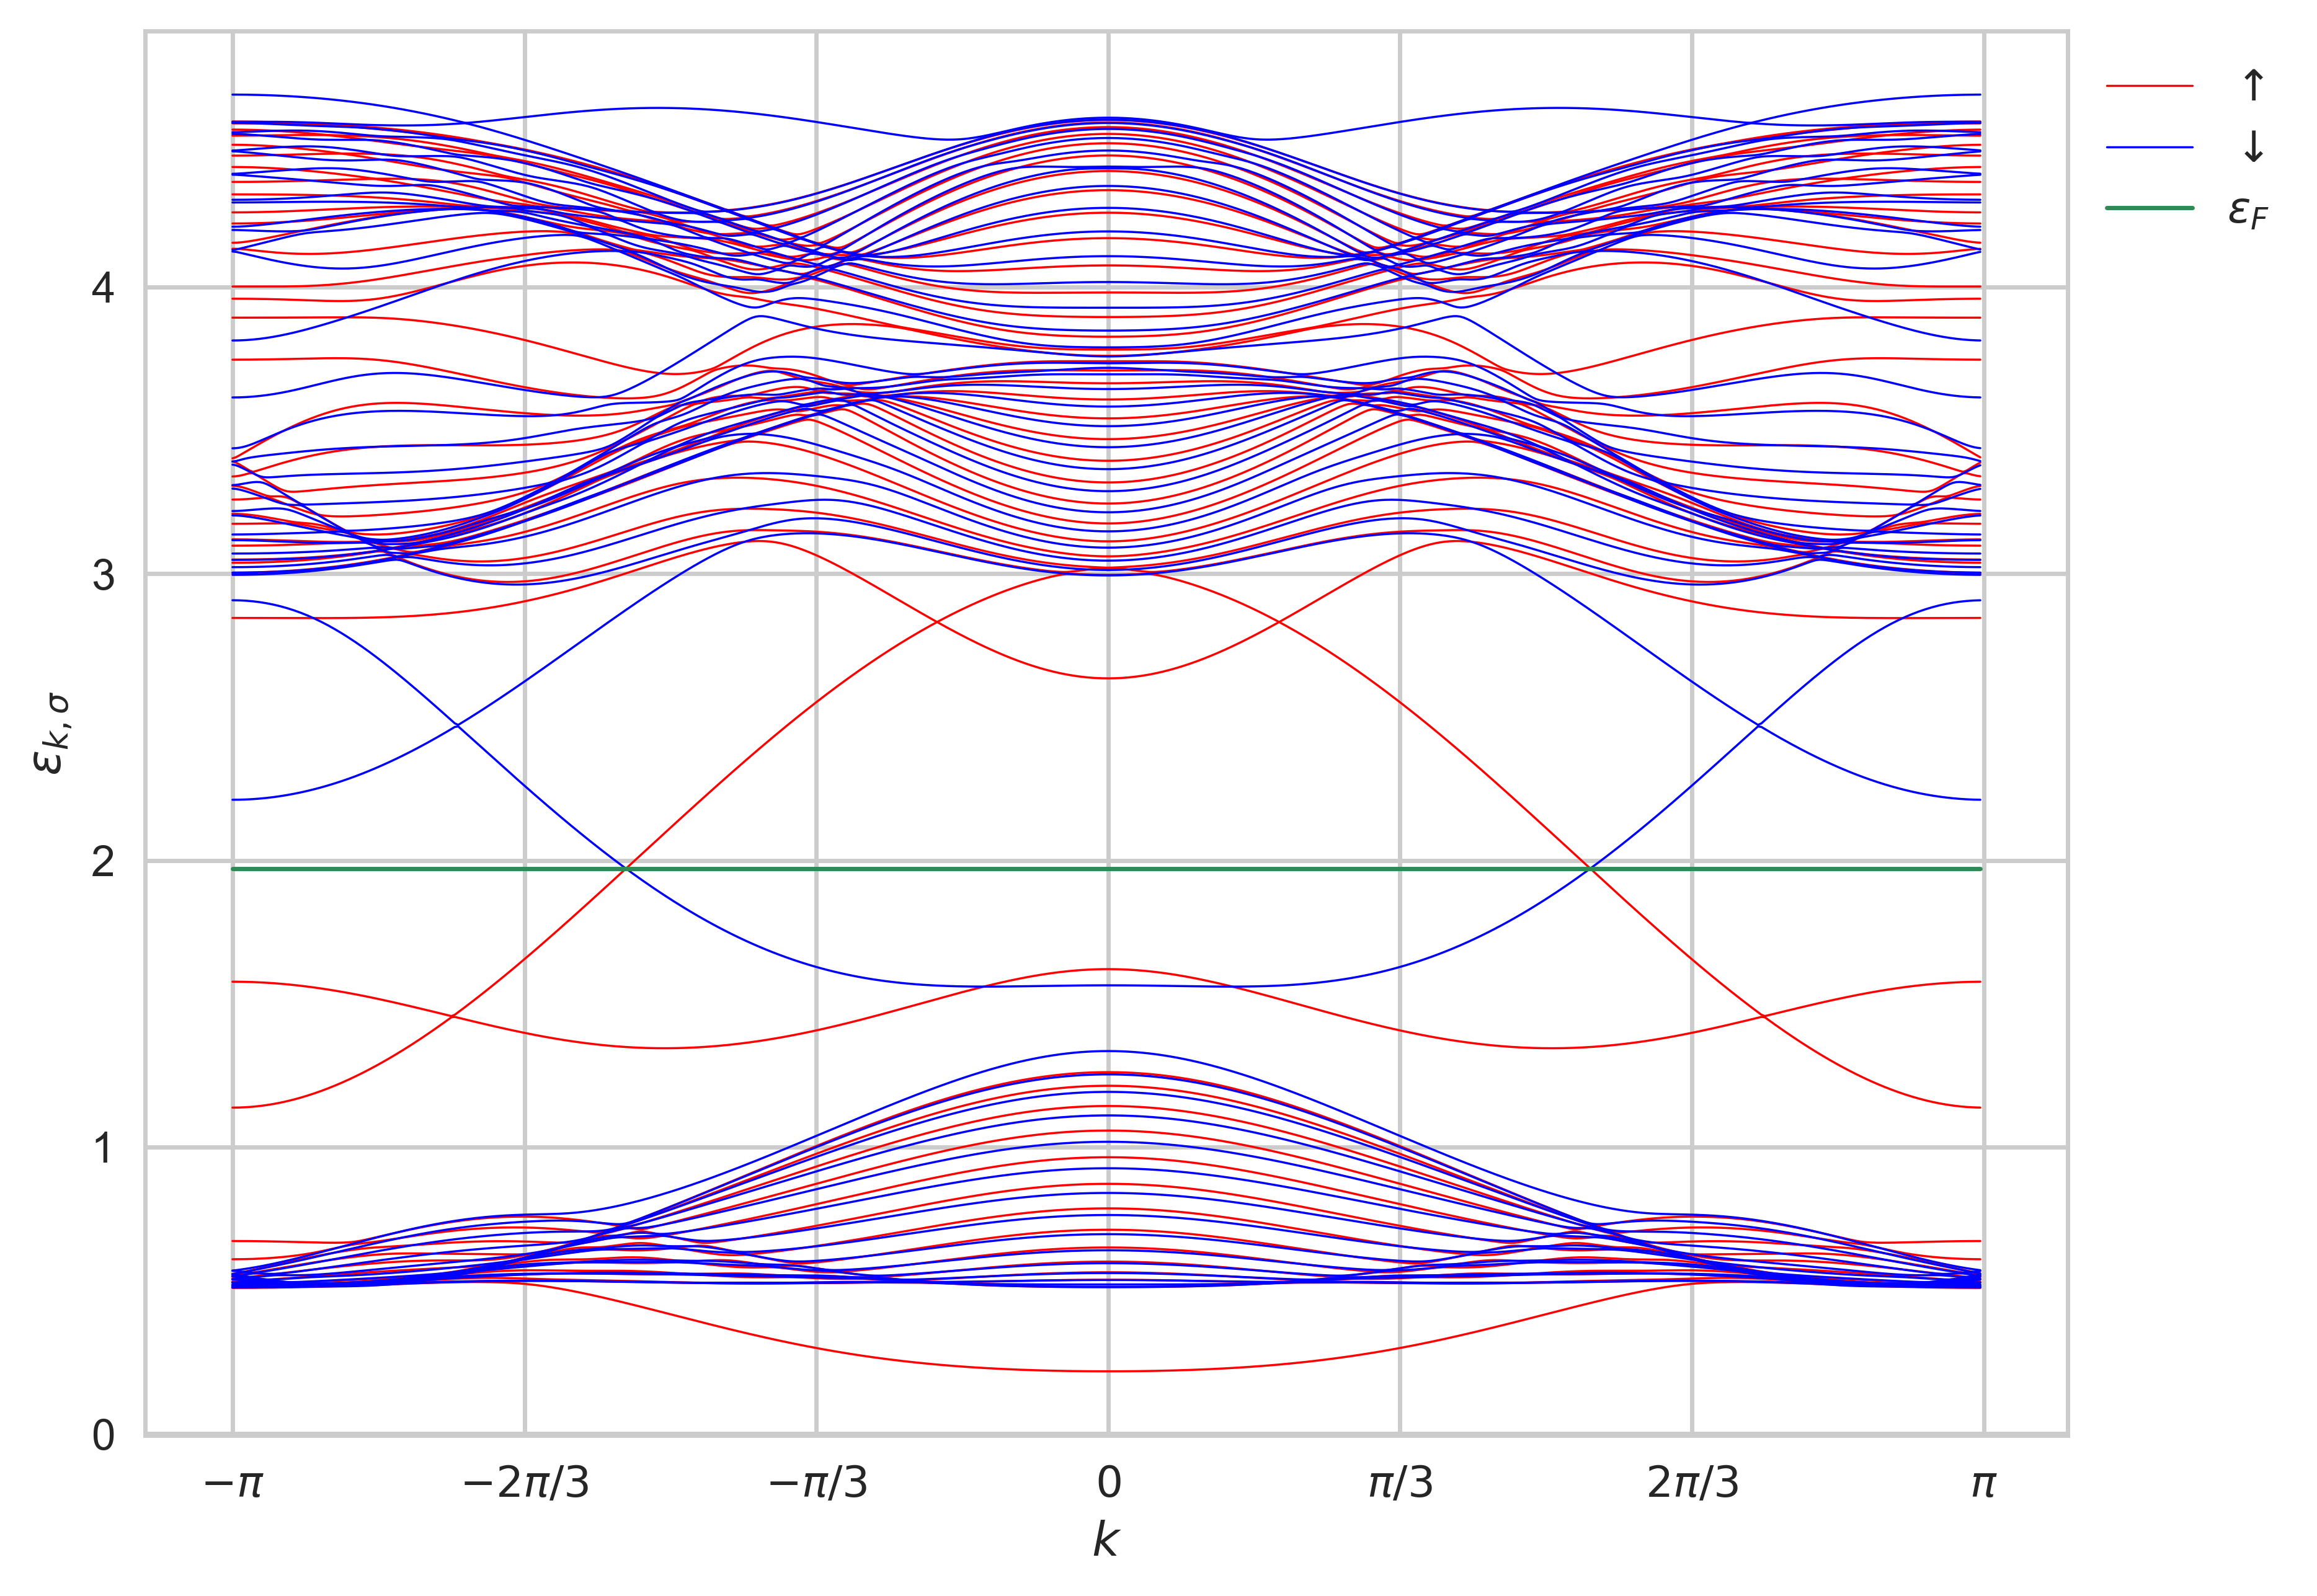
\includegraphics[scale = 0.42]{images/bands_Nx=512.png}
  \caption{Spin-resolved band structure within the ordered phase of a TMD nanoribbon of width $N_y = 16$, at $U = 20$.}
  \label{fig:bandsU20}
\end{figure}
\begin{figure}[H]
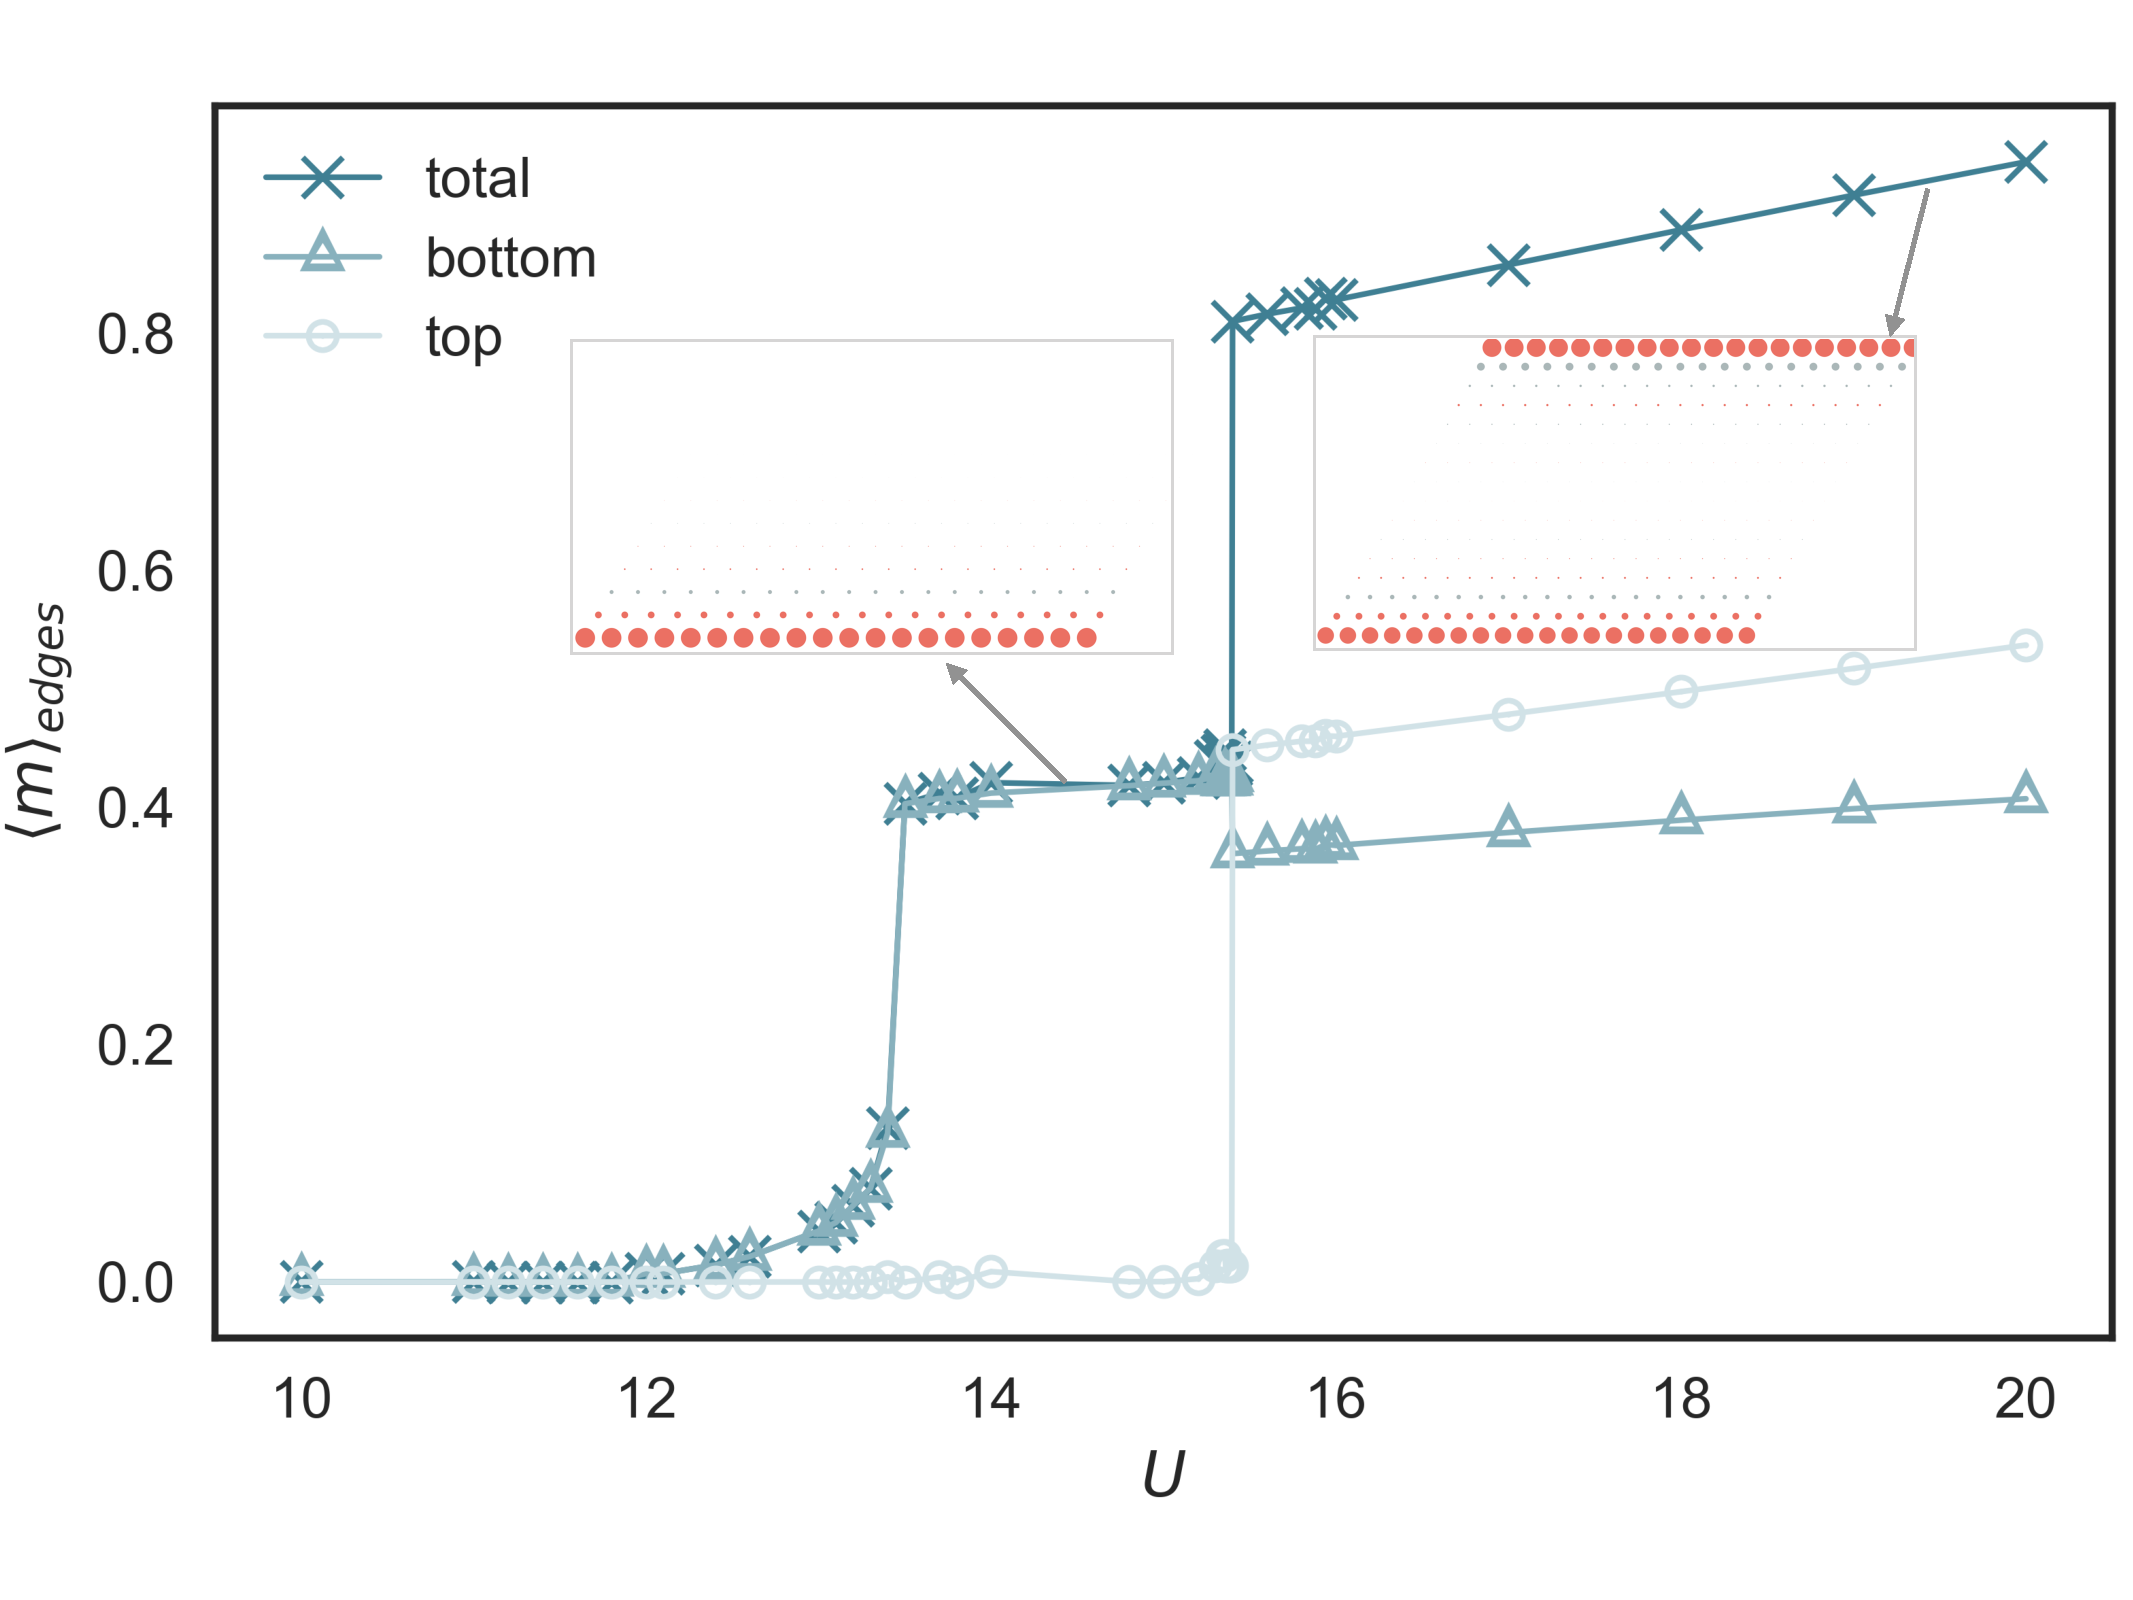
\includegraphics[trim={0cm 1.7cm 0cm 1.7cm},clip, scale =0.21]{images/edge-mag.pdf}
	\caption[Mean field phase diagram at zero temperature. Zoom-in of the first phase transition.]{Mean field phase diagram at zero temperature. Zoom-in of the first phase transition.
	\label{fig:zeroTphaseDiagram}}
\end{figure}
\begin{figure}[H]
\centering
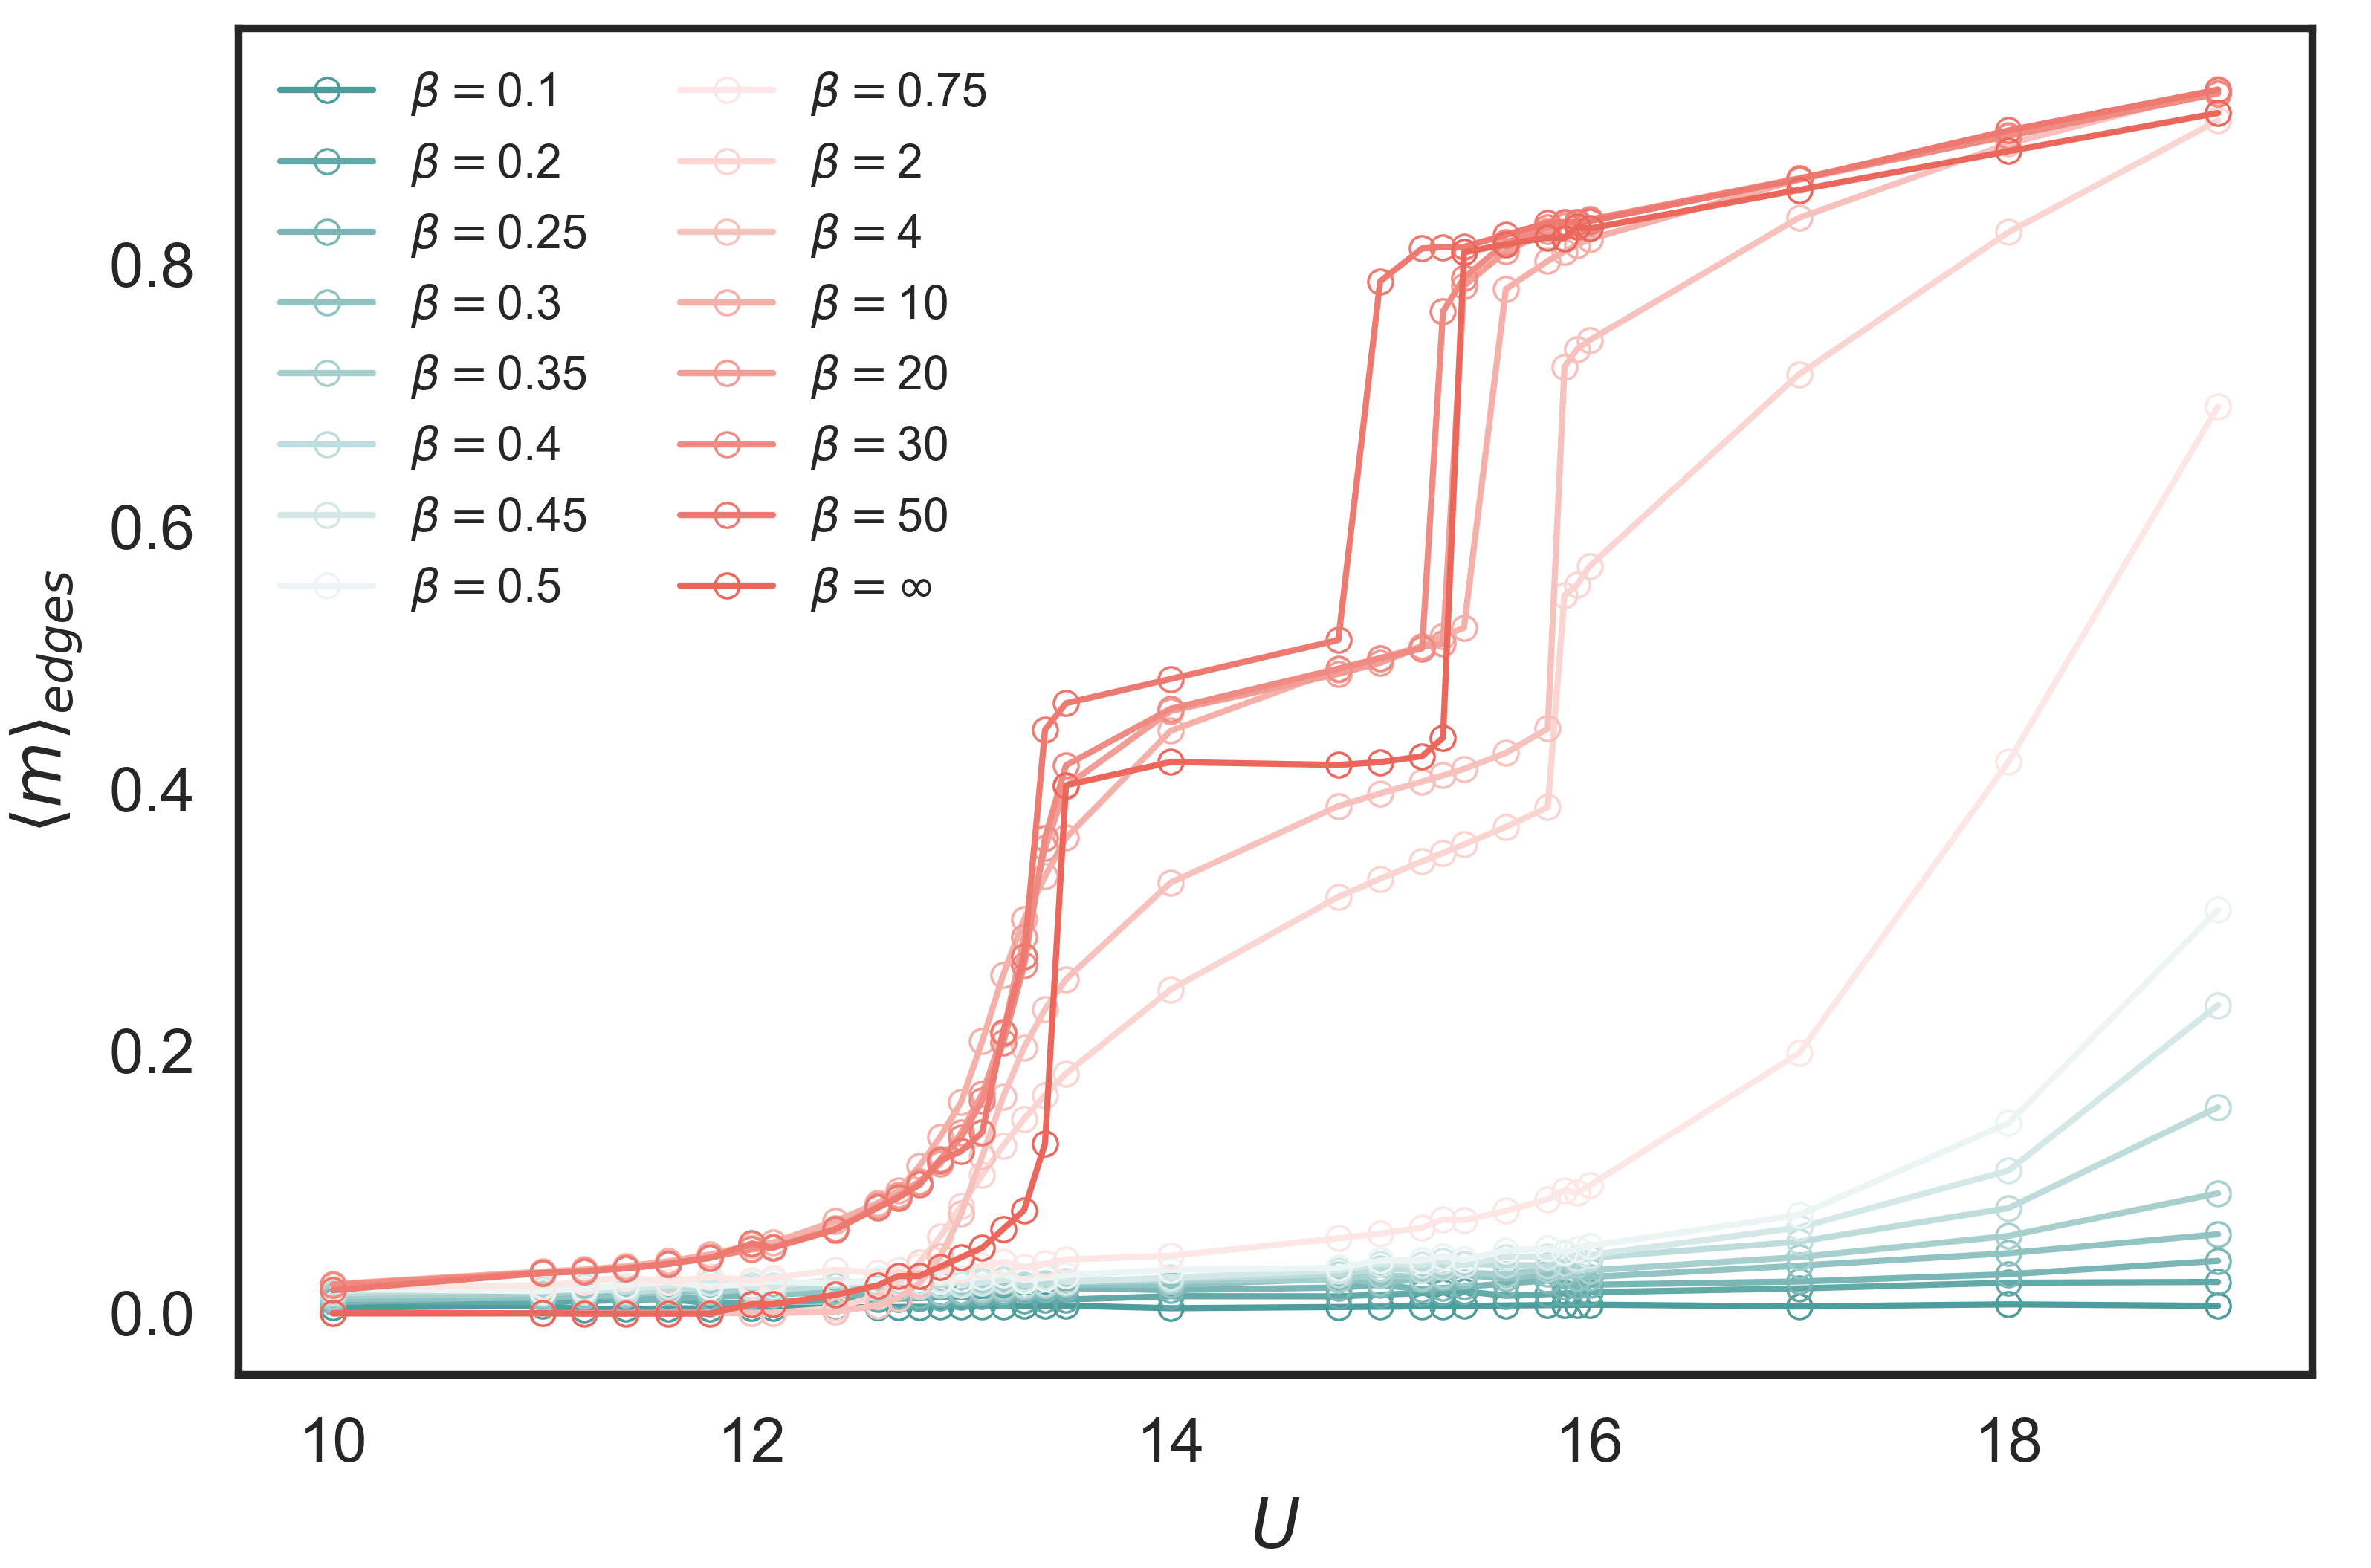
\includegraphics[width = 7.5cm]{images/edge-mag-phase-diagram.png}
	\caption[$T=0$ mean field band structure for a TMD nanoribbon of width $N_y = 16$ in the ordered phase, at $U=20 | t_0 |$.]{$T=0$ mean field band structure for a TMD nanoribbon of width $N_y = 16$ in the ordered phase ($U=20 | t_0 |$).}
	\label{fig:bandsZoomed}
\end{figure}
\begin{figure}[H]
    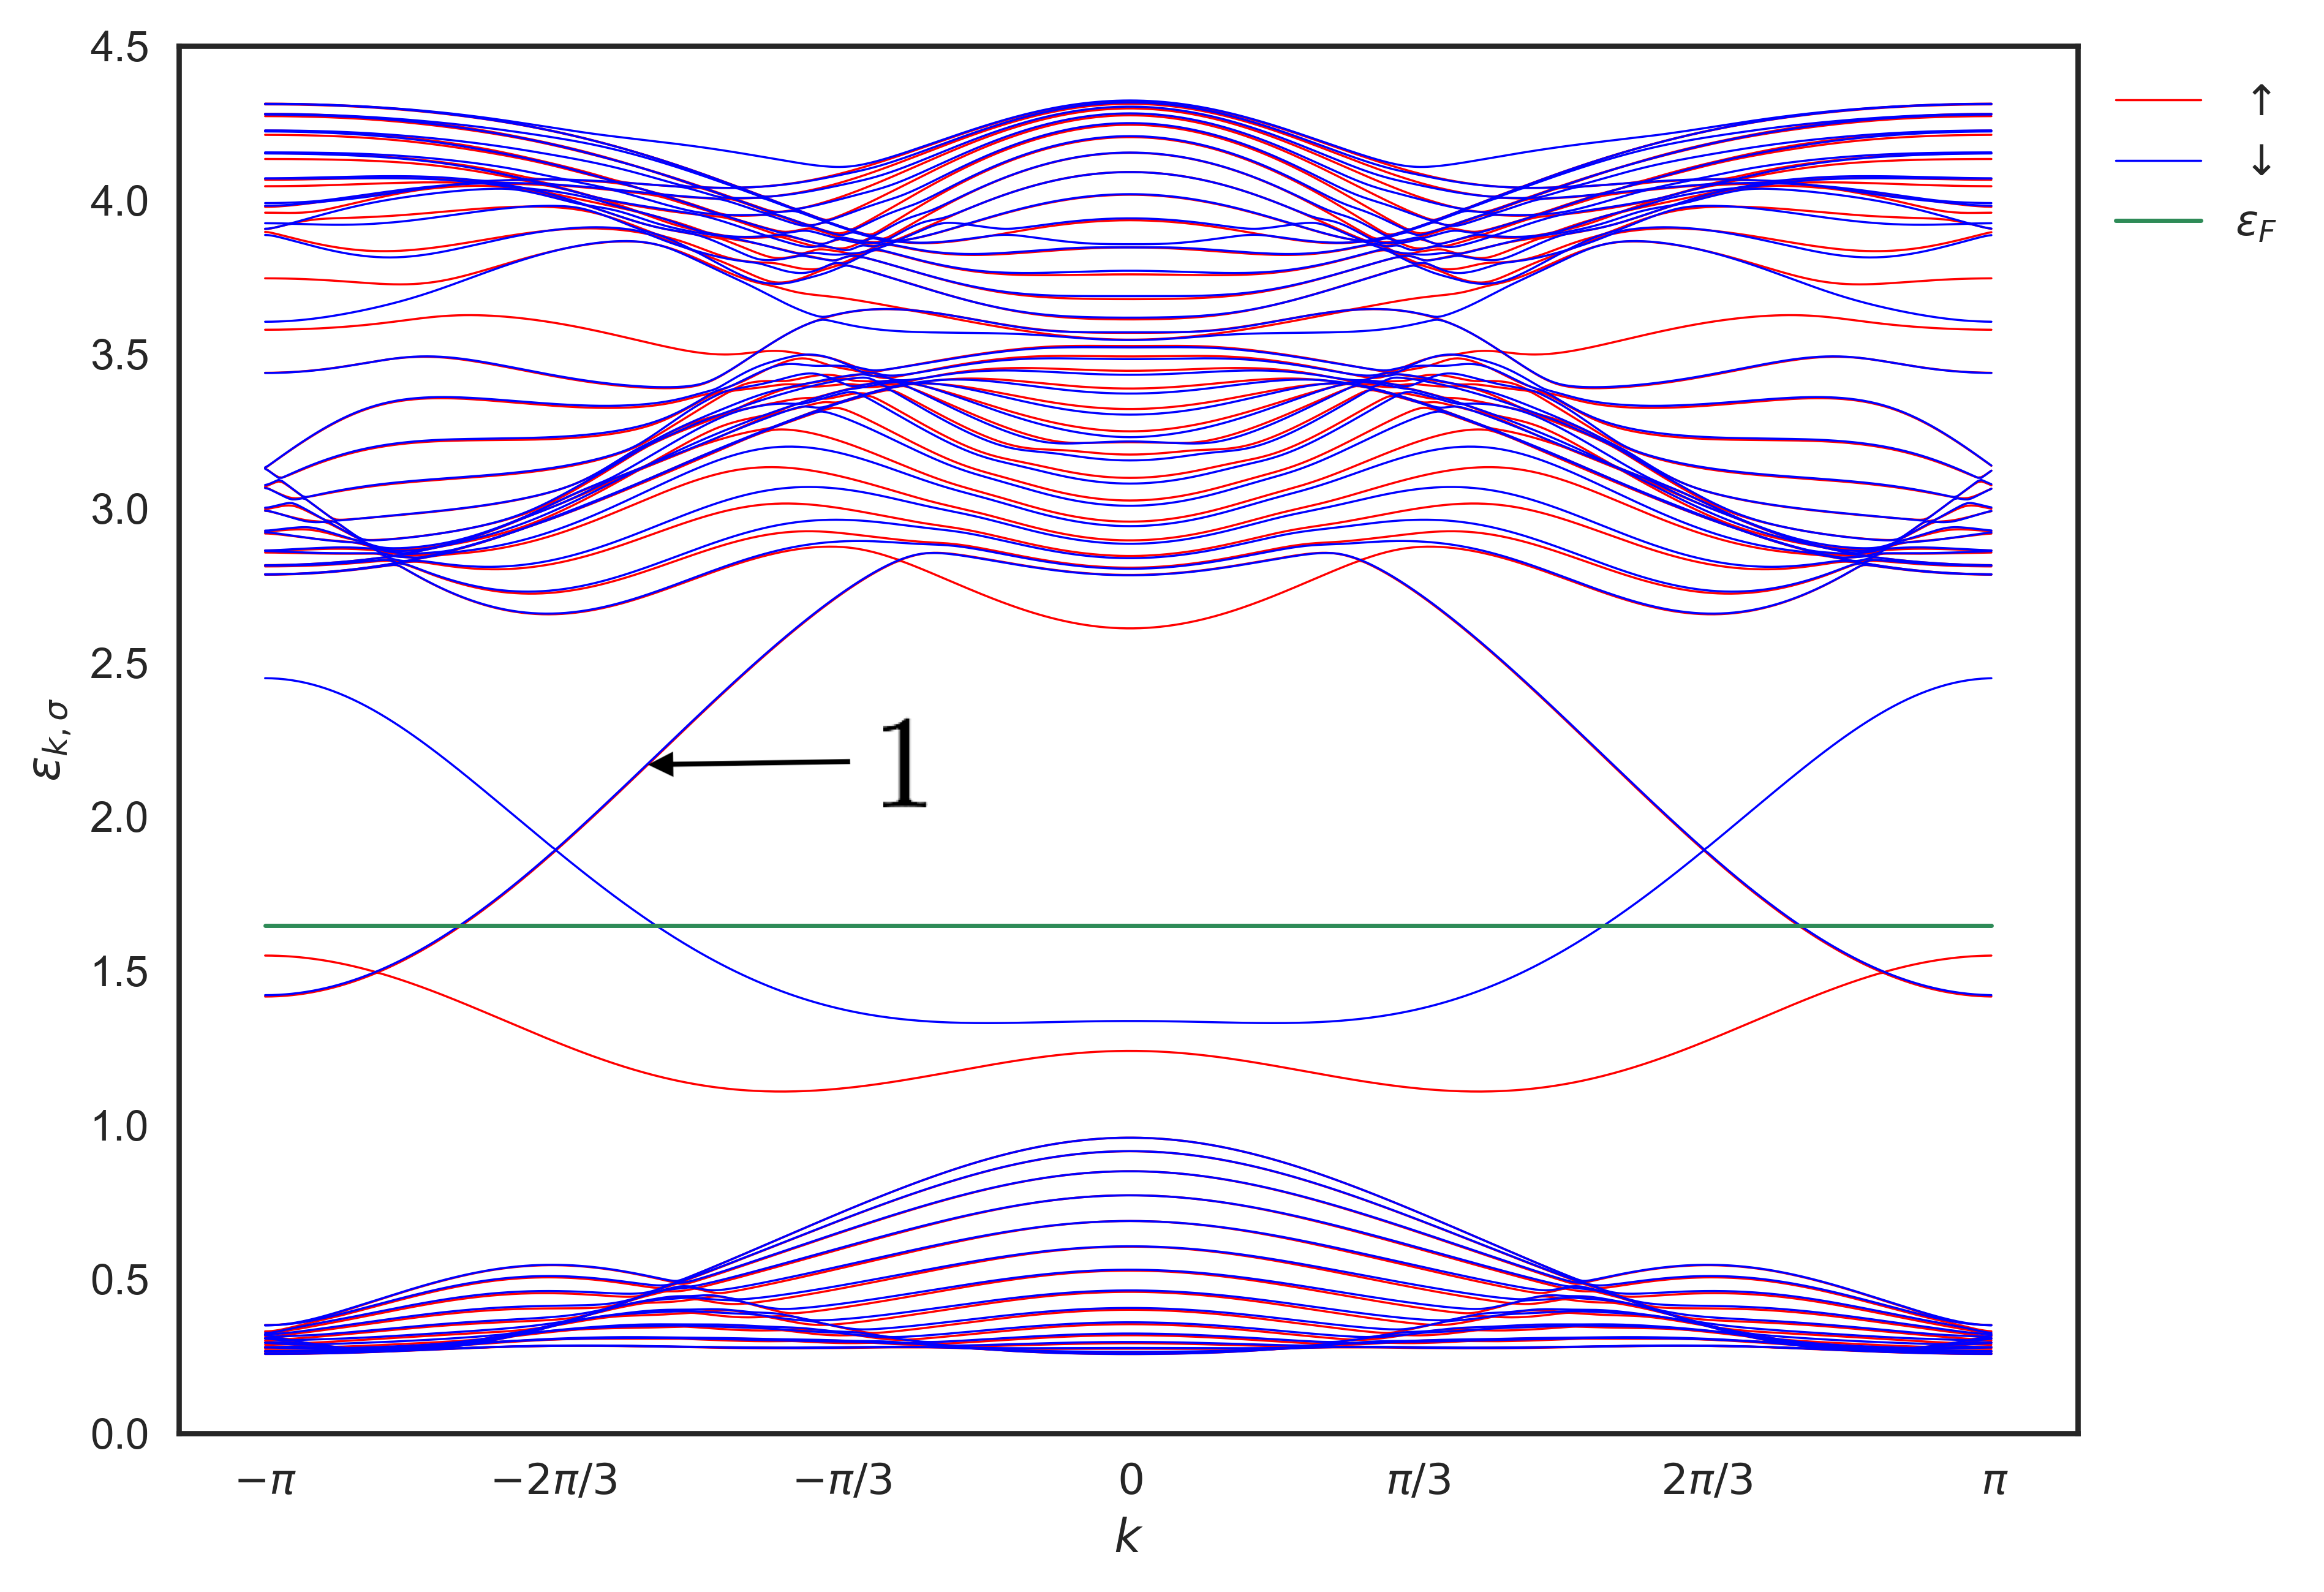
\includegraphics[width=6cm]{images/bands152.png}
  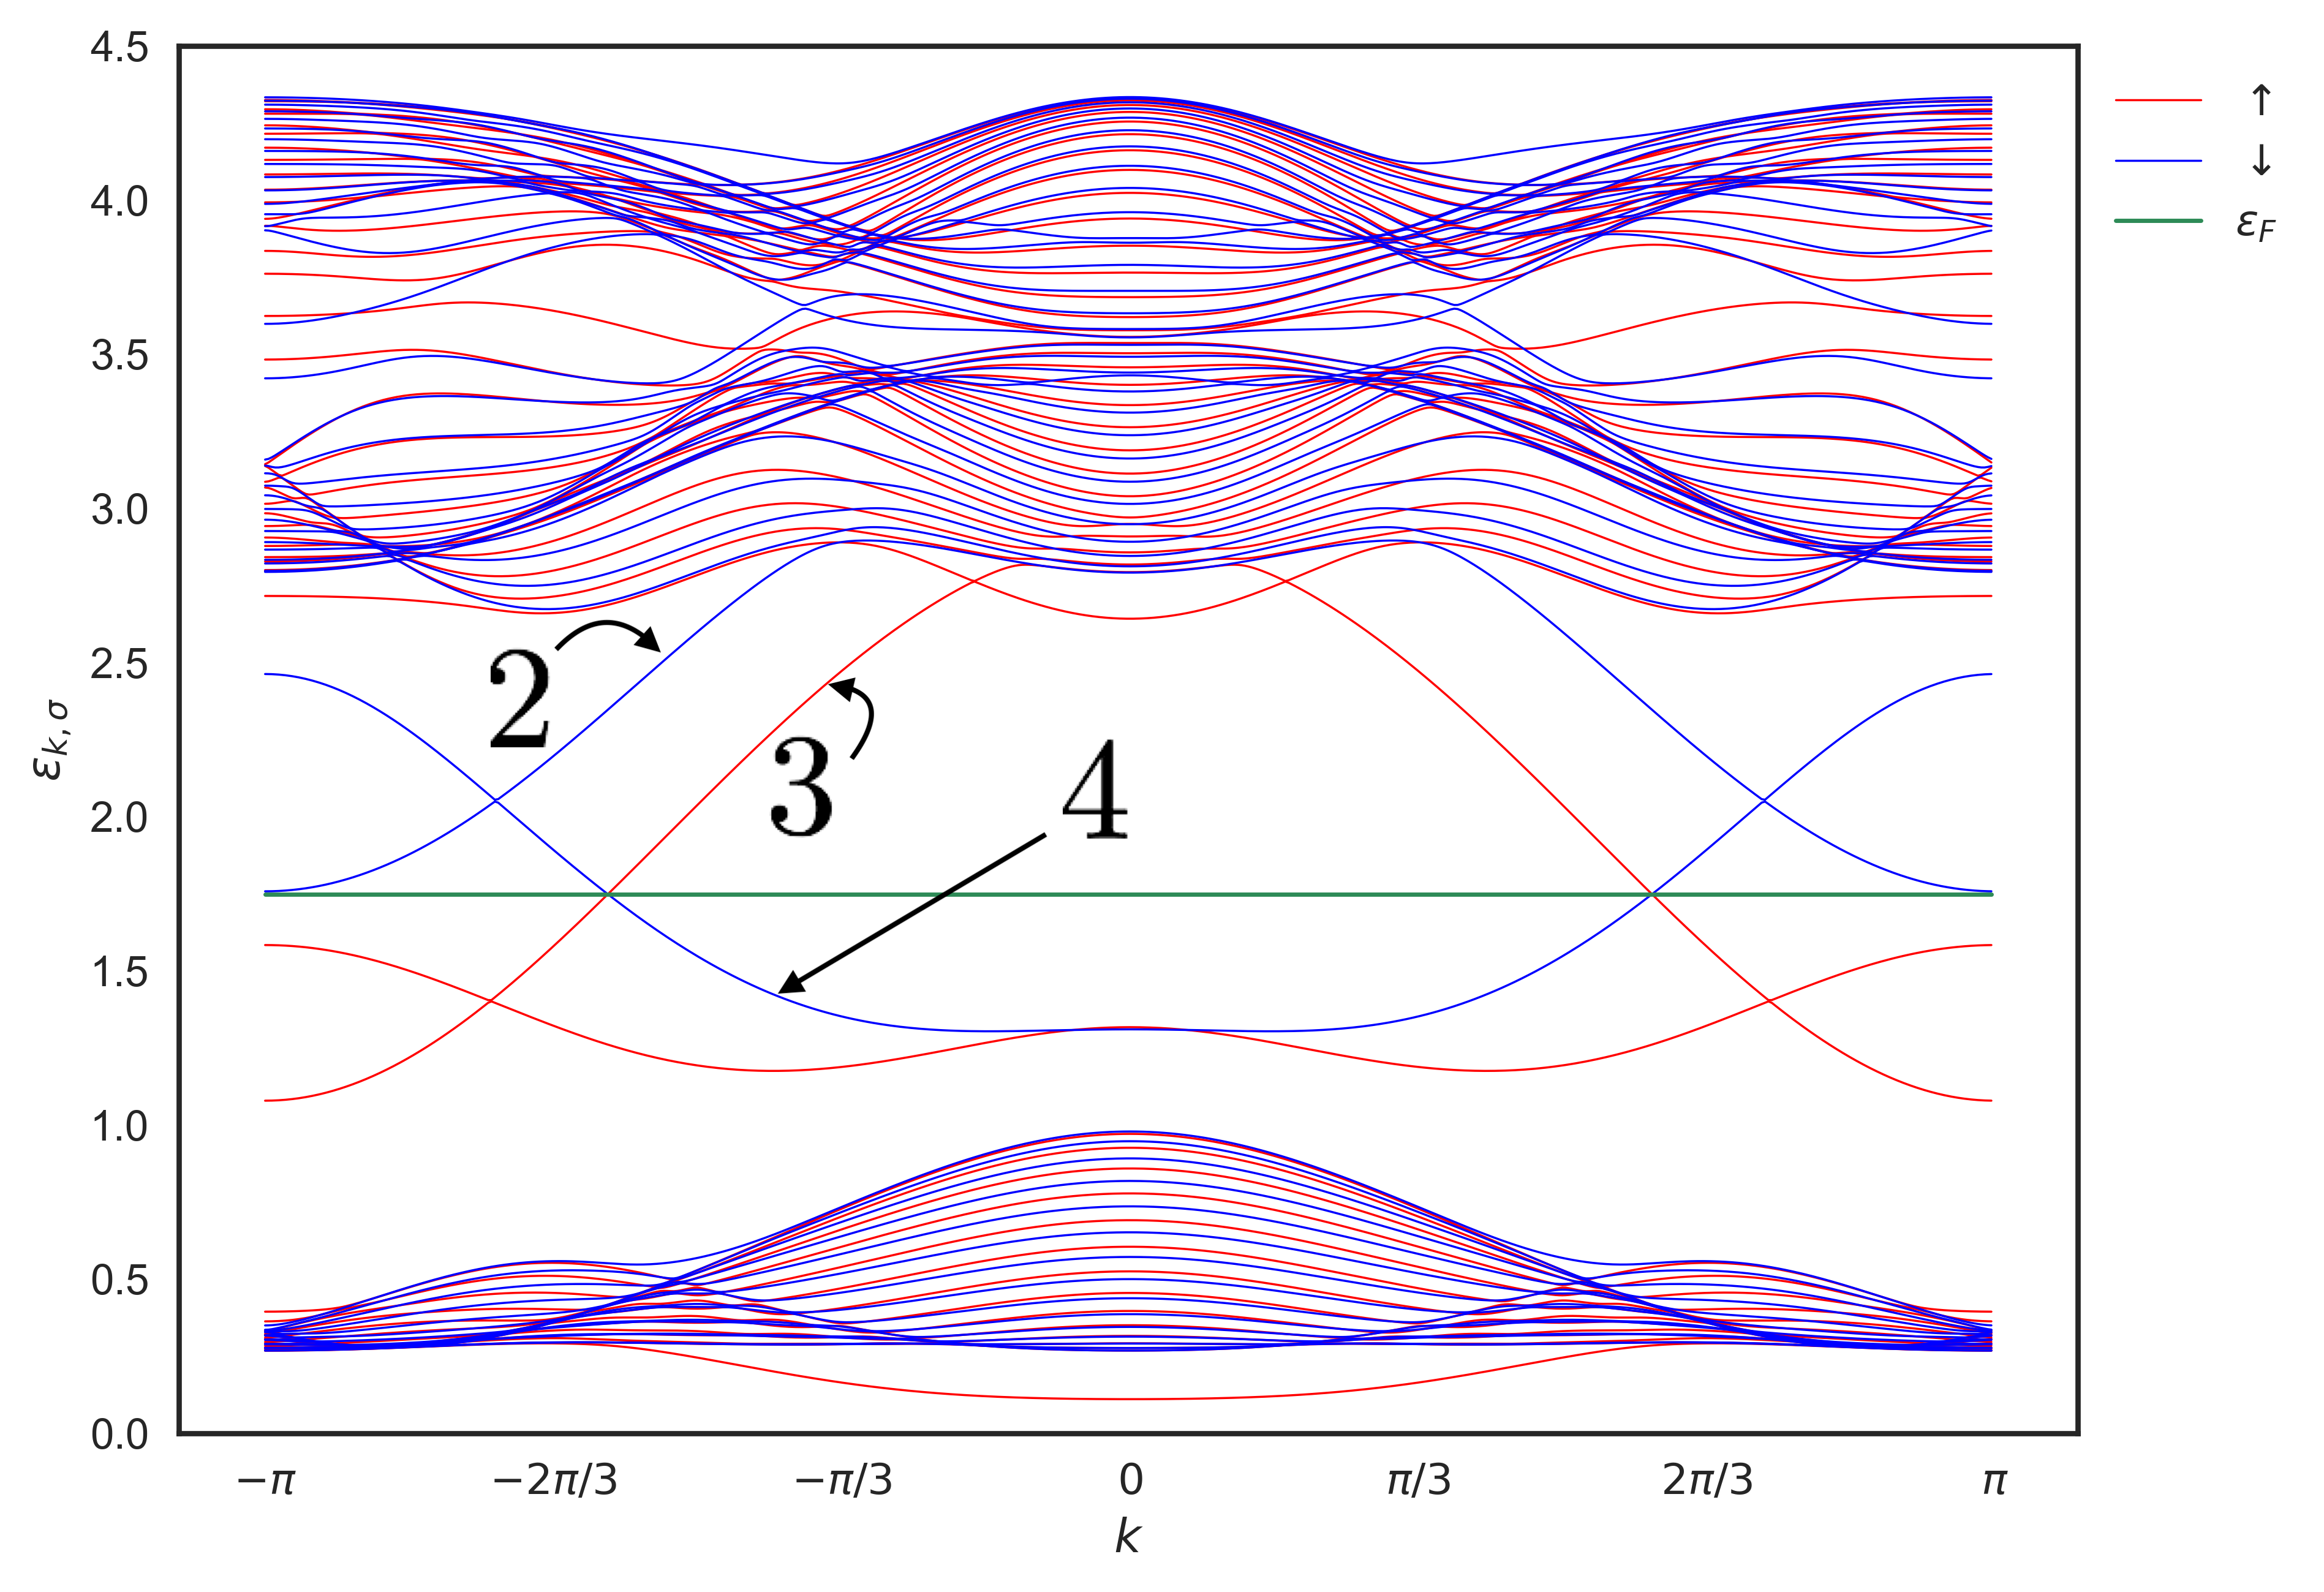
\includegraphics[width=6cm]{images/bands154.png}
  \caption{Comparison with \texttt{QUEST}}
  \label{fig:blade_flow_pressure}
\end{figure}
\begin{figure}[H]
  \centering
  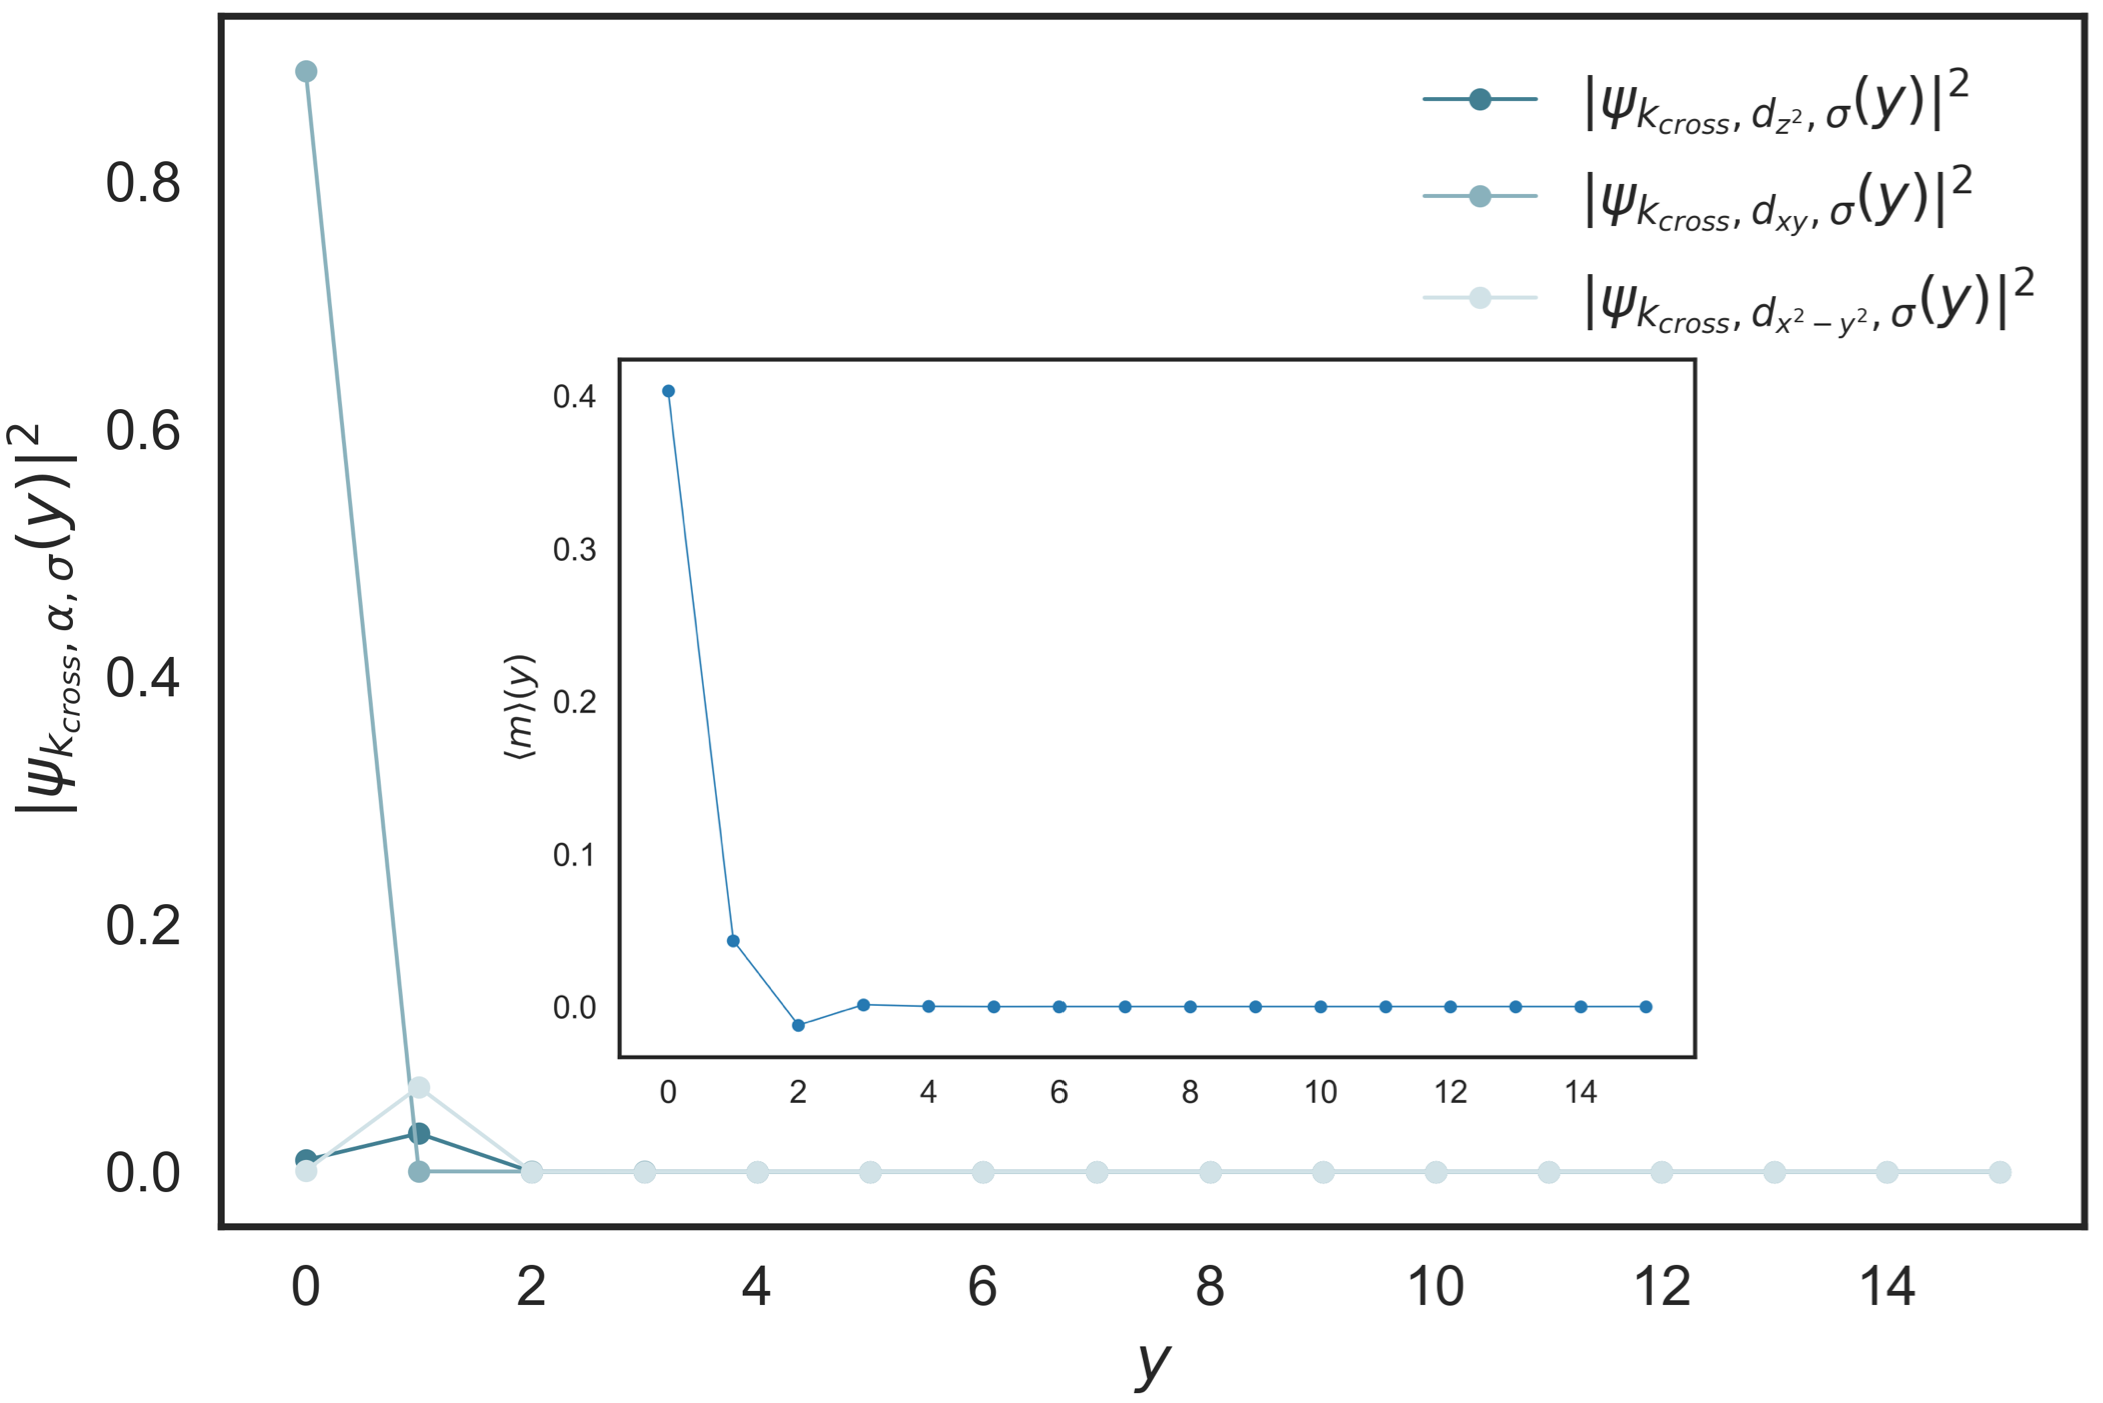
\includegraphics[width=6cm]{images/topEdgeMagProfU13.png}
  \caption{Comparison with \texttt{QUEST}}
  \label{fig:blade_flow_pressure}
\end{figure}
\begin{figure}[H]
  \centering
  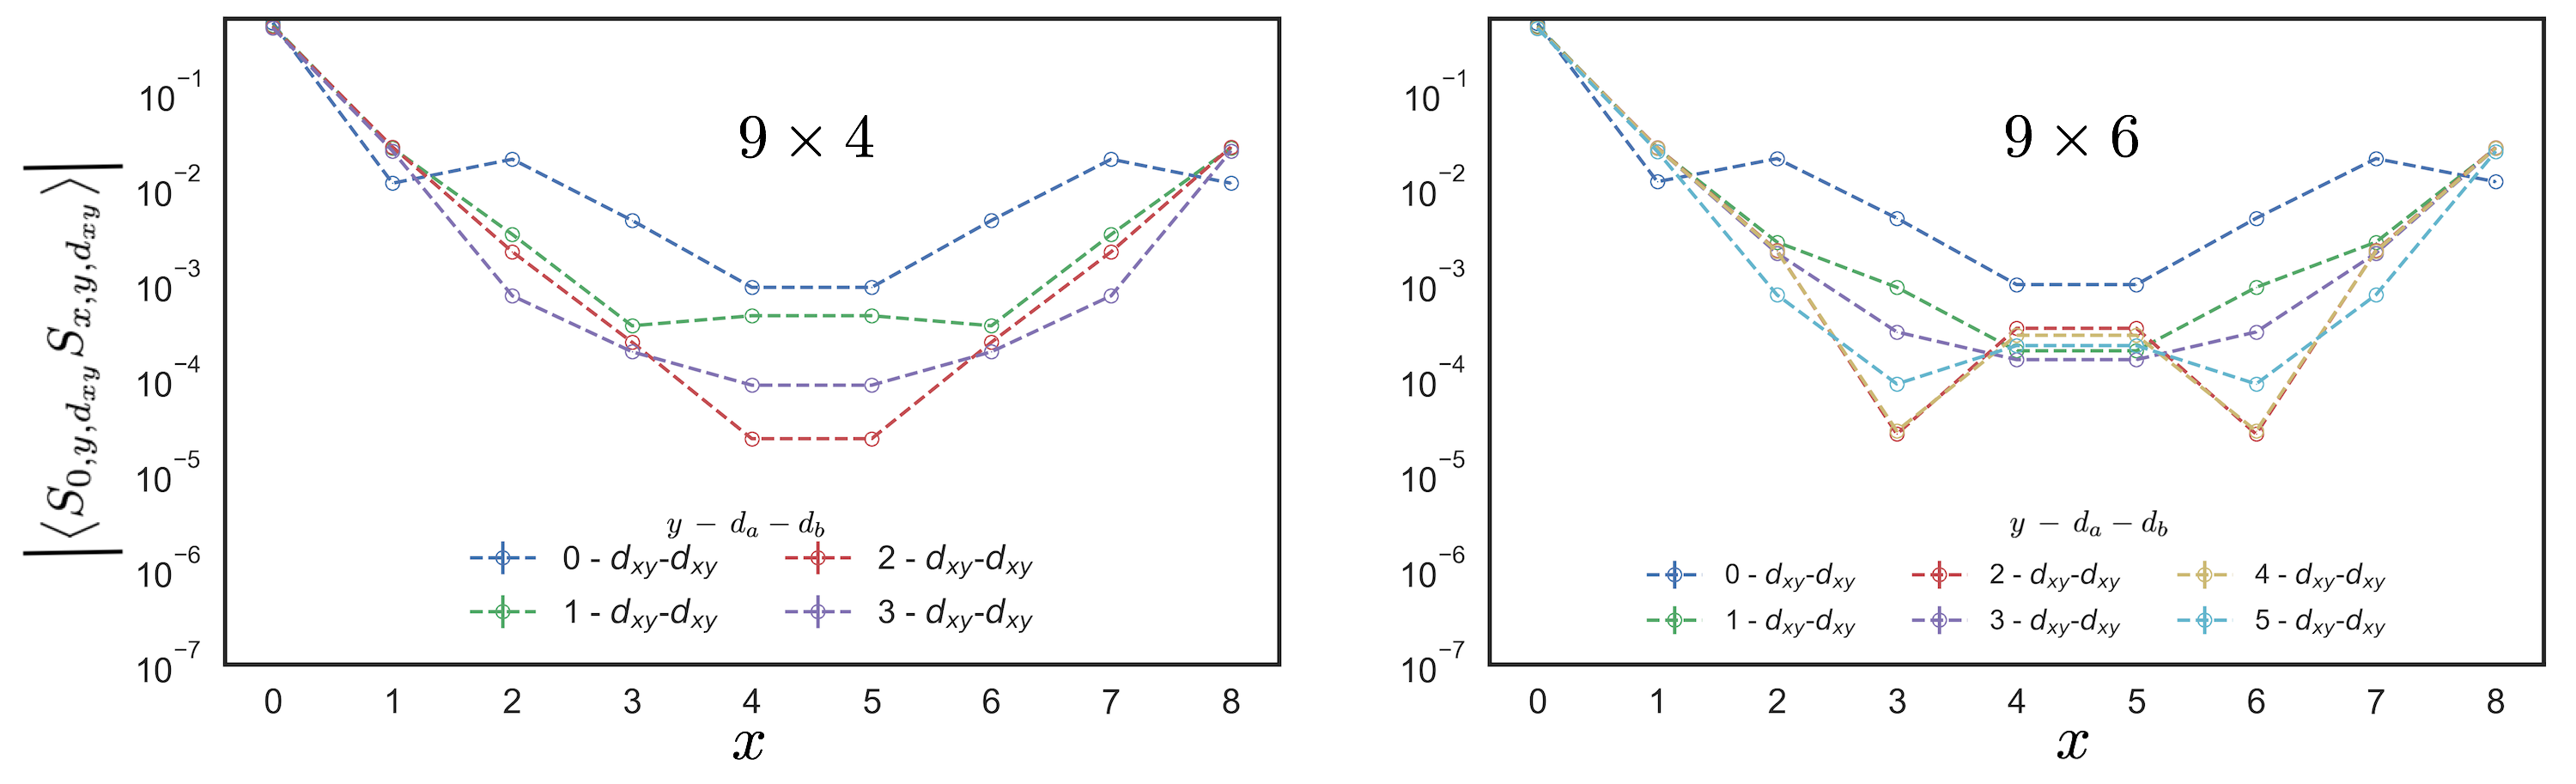
\includegraphics[width=7.5cm]{images/tmdFinalxyxy.png}
    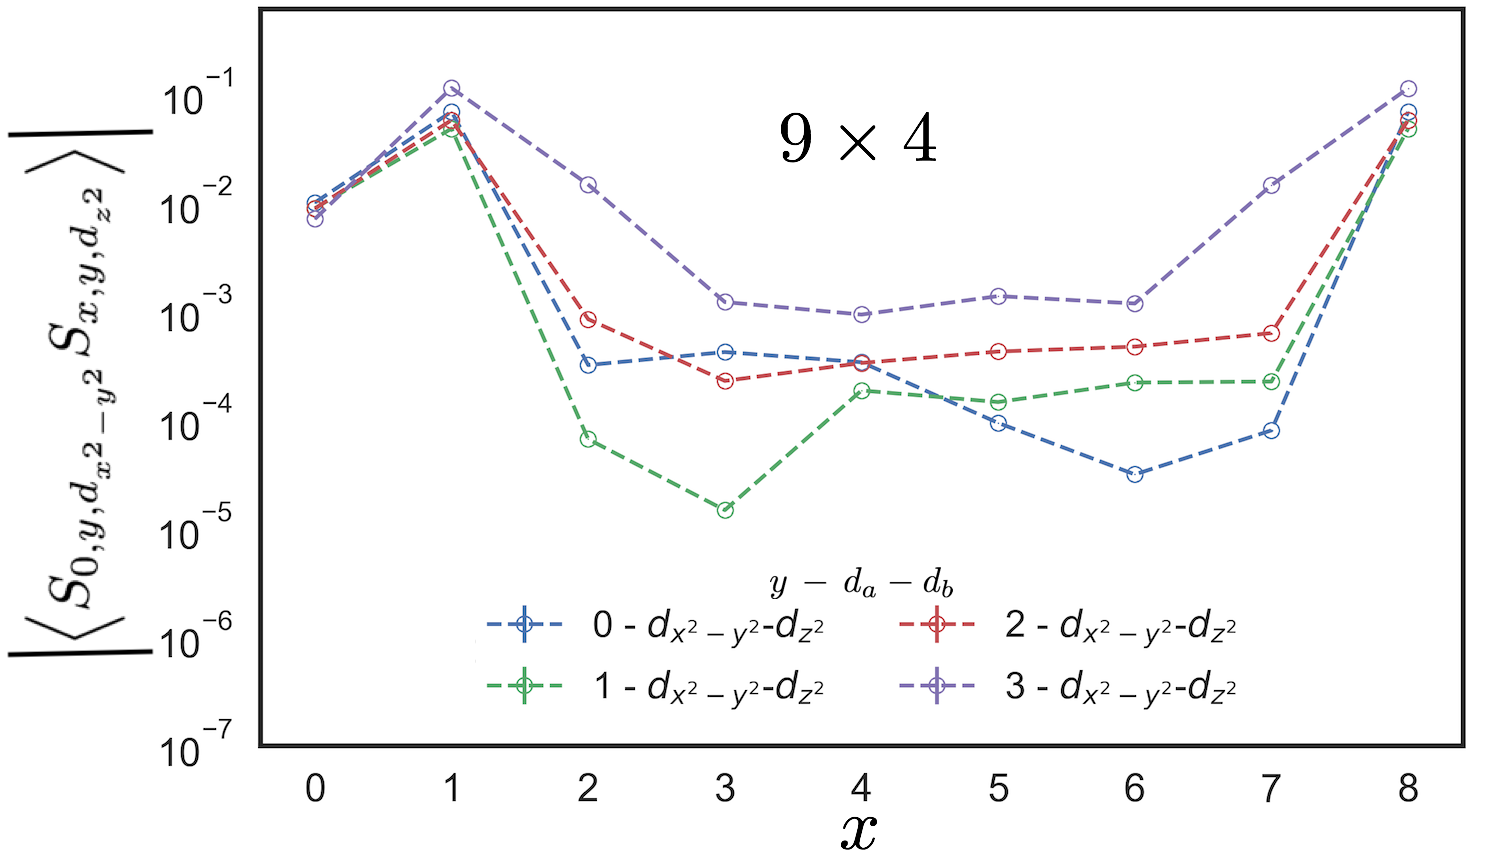
\includegraphics[width=7.5cm]{images/tmdFinalx2y2z2.png}
  \caption{Comparison with \texttt{QUEST}}
  \label{fig:blade_flow_pressure}
\end{figure}

%As seen in Fig.\ref{fig:blade_flow_pressure}...


%%%%%%%%%%%%%%%%%%%%%%%%%%%%%%%%%%%%%%%%%%%%%%%%%%%%%%%%%%%%%%%%%%%%%%
%\subsection{Sub-section...}

%More text...

%Table~\ref{table:simple} summarizes...

%\begin{table}[!h]
%  \begin{center}
%    \begin{tabular}{lccc}
%      Model           & $C_L$ & $C_D$ & $C_{M y}$ \\
%      \hline
%      Euler           & 0.083 & 0.021 & -0.110    \\
%      Navier--Stokes  & 0.078 & 0.023 & -0.101    \\
%      \hline
%    \end{tabular}
%  \end{center}
%  \caption[Table caption shown in TOC]{Table caption}
%  \label{table:simple}
%\end{table}

%As seen in Tab.\ref{table:simple}...

